% Copyright (c) 2023, Adam McKellar & Kai Rothe
% All rights reserved.
%
% This work is licensed under the Creative Commons Attribution 4.0 International License. To view a copy of this license, visit
% http://creativecommons.org/licenses/by/4.0/.

% !TEX engine = luatex
% !TeX spellcheck = en_EN


\documentclass{beamer}

\usepackage{amsmath}
\usepackage{amssymb}

\usepackage{hyperref}
\hypersetup{
	colorlinks,
	allcolors=.,
	urlcolor=blue,
}

\usepackage{fontspec}
\usepackage{polyglossia}
\setmainlanguage{english}

\usepackage{showexpl}

\usepackage[useregional]{datetime2}

% https://hartwork.org/beamer-theme-matrix/
\usetheme{Antibes}
\usecolortheme{beaver}
\useinnertheme{circles}

% pseudocode: 
\usepackage[vlined]{algorithm2e}
\DontPrintSemicolon
\SetKw{KwCont}{continue}

% images:
\usepackage{wrapfig}

\usepackage[
	type={CC},
	modifier={by},
	version={4.0},
	imagemodifier={-80x15},
]{doclicense}


\author{Adam McKellar\qquad Kai Rothe\qquad\quad}
\title{Feedback Arc Set in Tournaments}
\date{June 22, 2023} % date of presentation

\newcommand{\abs}[1]{\left| #1 \right|}

\begin{document}
	\frame{\titlepage}
	
	\begin{frame}{Overview}
		\tableofcontents
		\tiny
		\doclicenseThis
	\end{frame}


	\section{Feedback Arc Set in Tournaments}
	\begin{frame}[fragile]{Feedback Arc Set (FAS)}
		\begin{align*}			
			FAS := \{&(G = (V, E), k) | G \text{ is directed } \\
										&\land \exists E' \subset E : \abs{E'} \leq k : G' = (V, E - E') \text{ is acyclic}  \}		
		\end{align*}
	\end{frame}
	\begin{frame}[fragile]{Feedback Arc Set (FAS) Example}
		Example \(G\) :
		\begin{center}
			\includegraphics<1>[height=0.3\paperheight]{images/FAS/cyclic_graph_example.pdf}
			\includegraphics<2>[height=0.3\paperheight]{images/FAS/cyclic_graph_example_highlight_cycles.pdf}
			\includegraphics<3>[height=0.3\paperheight]{images/FAS/cyclic_graph_example_highlight_solution_k2.pdf}
			\includegraphics<4->[height=0.3\paperheight]{images/FAS/cyclic_graph_example_highlight_solution_k1.pdf}
		\end{center}
		\begin{itemize}
			\item<3-> Solvable for \(k=2\)
			\item<4-> Solvable for \(k=1\)
			\item<5-> \(\Rightarrow (G, 1) \in FAS\)
		\end{itemize}
	\end{frame}

	\begin{frame}[fragile]{Tournaments (T)}
		\begin{center}
			\includegraphics<1>[height=0.3\paperheight]{images/T/complete_graph_example.pdf}
			\includegraphics<2->[height=0.3\paperheight]{images/T/tournament_example.pdf}
		\end{center}
		\begin{itemize}
			\item<1-> Take a complete graph.
			\item<2-> Assign every edge a direction.
			\item<3-> \(T := \{ (G = (V, E)) | \forall u, v \in V : (u, v) \in E \veebar (v, u) \in E \}\)
		\end{itemize}
	\end{frame}
	\begin{frame}[fragile]{Feedback Arc Set in Tournaments (FAST)}
		\[	FAST := \{ (G = (V, E), k) | G \in T \land (G, k) \in FAS \} \]
		\begin{center}
			\includegraphics<2>[height=0.3\paperheight]{images/T/tournament_example.pdf}
			\includegraphics<3->[height=0.3\paperheight]{images/FAST/fast_example.pdf}
		\end{center}
		\begin{itemize}
			\item<3-> \((G, 1)\in FAST\)
		\end{itemize}
	\end{frame}


	\section{Lemma 2.5 (without proof)}
	\begin{frame}[fragile]{Lemma 2.5}
		For a directed graph \(G\)
		\[ G \text{ is acyclic } \Leftrightarrow  \forall (u,v) \in E(G) : u < v \]
		\begin{center}
			\includegraphics<2-3>[height=0.3\paperheight]{images/Lemma25/acyclic_graph.pdf}
			\includegraphics<4->[height=0.3\paperheight]{images/Lemma25/cyclic_graph.pdf}
		\end{center}
		
		\only<3>{ \(V = \{a, b, c, d\}\) \qquad \(E = \{(a, b), (b, c), (c, d), (a, d)\}\) \\
			\(\Rightarrow a < b \land b < c \land c < d \land a < d \Rightarrow a < b < c < d \Rightarrow \text{ acyclic}\)	}
	
		\only<5->{ \(V = \{a, b, c, d\}\) \qquad \(E = \{(a, b), (b, c), (c, d), \color{red} (d, a) \color{black} \}\) \\
			\(\Rightarrow a < b \land b < c \land c < d \land \color{red} d < a \color{black} \Rightarrow a < d \land  \color{red} d < a \color{black} \Rightarrow \text{ no total order } \Rightarrow \text{ cyclic }\) }
	\end{frame}
	

	\section{Observation 2.6}
	\begin{frame}[fragile]{\(\circledast\)}
		\begin{center}
			\includegraphics<1>[height=0.3\paperheight]{images/CircledAsterix/graph_G.pdf}
			\includegraphics<2>[height=0.3\paperheight]{images/CircledAsterix/edges_f.pdf}
			\includegraphics<3>[height=0.3\paperheight]{images/CircledAsterix/edges_revF.pdf}
			\includegraphics<4>[height=0.3\paperheight]{images/CircledAsterix/graph_GrevF.pdf}
		\end{center}
		\begin{itemize}[<+->]
			\item \(G = (V, E)\)
			\item \(F \subseteq E(G)\)
			\item \(rev(F) := \{(u, v) : (v, u) \in F\}\)
			\item \[ G\circledast F := (V(G), \left( E(G) \cup rev(F) \right)\setminus F ) \]
		\end{itemize}
	\end{frame}

	\begin{frame}[fragile]{Observation 2.6}
		\begin{center}
			\includegraphics<1>[height=0.3\paperheight]{images/Observation26/cyclic_graph_with_F.pdf}
			\includegraphics<2>[height=0.3\paperheight]{images/Observation26/acyclic_G_ast_F.pdf}
			\includegraphics<3>[height=0.3\paperheight]{images/Observation26/acyclic_G_without_FAS.pdf}
		\end{center}
		\only<+->{\[ 
			F \subseteq E(G)	
		\]}
		\only<+->{\[ 
			\text{if } G\circledast F \text{ is a directed acyclic graph}
		\]}
		\only<+->{\[ 
			\Rightarrow F \text{ is a feedback arc set of } G	
		\]}
	\end{frame}
	\begin{frame}[fragile]{Observation 2.6 \textit{ is implied by Lemma 2.5 }}
		\begin{center}
			\includegraphics<1>[height=0.3\paperheight]{images/Observation26/cyclic_graph_with_F.pdf}
			\includegraphics<2>[height=0.3\paperheight]{images/Observation26/acyclic_G_ast_F.pdf}
			\includegraphics<3>[height=0.3\paperheight]{images/Observation26/acyclic_G_without_FAS.pdf}
		\end{center}
		
		\only<1>{ \(V = \{a, b, c, d\}\) \qquad \(E = \{(a, b), (b, c), (c, d), \color{red} (d, a) \color{black} \}\) \\
			\(\Rightarrow a < b \land b < c \land c < d \land \color{red} d < \dotsc \color{black} \Rightarrow \text{ no total order } \Rightarrow \text{ cyclic }\) }
	 	\only<2-3>{\(V = \{a, b, c, d\}\) \qquad \((E\cup rev(F))\setminus F = \{(a, b), (b, c), (c, d), \color{blue}(a, d) \color{black} \}\) \\
			\(\Rightarrow a < b \land b < c \land c < d \land \color{blue} a < d \color{black} \Rightarrow a < b < c < d \Rightarrow \text{ acyclic}\)}
		\only<3>{\[ \Rightarrow   a < b \land b < c \land c < d \Rightarrow a < b < c < d \Rightarrow \text{ acyclic}\]}
		
	\end{frame}
	
	
	\section{Lemma 2.7}
	\begin{frame}[fragile]{Lemma 2.7}
		\begin{align*}
			&\qquad F \in min \left\{ F' \subset E(G) | F' \text{ is a Feedback Arc Set of } G \right\} \\
			&\Leftrightarrow \\
			&\qquad F \in min \left\{ F' \subset E(G) | G\circledast F' \text{ is acyclic} \right\}
		\end{align*}	
	\end{frame}
	
	\section{Lemma 2.7 \(\Rightarrow\)}
	\begin{frame}[fragile]{Lemma 2.7 ``\(\Rightarrow\)''}
		\begin{align*}
			&\qquad F \in min \left\{ F' \subset E(G) | F' \text{ is a Feedback Arc Set of } G \right\} \\
			&\Rightarrow \\
			&\qquad F \in min \left\{ F' \subset E(G) | G\circledast F' \text{ is acyclic} \right\}
		\end{align*}	
	\end{frame}
	\begin{frame}[fragile]{Lemma 2.7 ``\(\Rightarrow\)'' \--- Assumptions}
		\begin{center}
			\includegraphics<1-2>[height=0.3\paperheight]{images/Lemma27/Abstract_Graph_G_with_Edge_of_F.pdf}
			\includegraphics<3>[height=0.3\paperheight]{images/Lemma27/Abstract_Graph_G_without_F.pdf}
			\includegraphics<4->[height=0.3\paperheight]{images/Lemma27/Abstract_Graph_G_with_Edge_of_revF_and_Cycle_C.pdf}
		\end{center}
		\begin{enumerate}
			\item<1-> \(  F \in min \left\{ F' \subset E(G) | F' \text{ is a Feedback Arc Set of } G \right\} \)
			\item<2-> let \(e_1, \dotsc , e_n \in F \)
			\item<3-> \(\Rightarrow G' = \left(V(G), E(G)\setminus F\right) \) is acyclic
			\item<4-> \textbf{Assumption:} \( G\circledast F \) has a cycle \( C \)
			\item<5-> \(\Rightarrow E(C) \cup \left(E(G)\setminus F\right) \neq \left(E(G)\setminus F\right)\)
			\item<6-> \(\Rightarrow \exists f \in E(C) : f\in rev(F)\)
			%\item<7-> let \(f_1, \dotsc , f_l \in \left(C \cap rev(F)\right) \neq \emptyset\)
		\end{enumerate}
	\end{frame}
	\begin{frame}[fragile]{Lemma 2.7 ``\(\Rightarrow\)'' \--- Contradiction}
		\begin{center}
			\includegraphics<1-2>[height=0.3\paperheight]{images/Lemma27/Abstract_Graph_G_with_Edge_of_F_and_Cylce_of_G.pdf}
			\includegraphics<3>[height=0.3\paperheight]{images/Lemma27/Abstract_Graph_G_with_Edge_of_revF_and_Cycle_C.pdf}
			\includegraphics<4->[height=0.3\paperheight]{images/Lemma27/Abstract_Graph_G_with_C_and_C_of_i.pdf}
		\end{center}
		\begin{itemize}[<+->]
			\item let \(C_i\) with \(1\leq i \leq n\) be cycles in \(G\)
			\item \( F\text{ is minimal } \Rightarrow F \cap E(C_i) = \{e_i\} \)
		\end{itemize}
		\begin{enumerate}[<+->]
		 	\item Traverse \(C\) in \(G\)
		 	\item Instead of traversing \(f_i := rev(e_i)\), we traverse \(C_i - e_i\)
		 	\item \(C\) can be traversed without edges of \(rev(F)\) or \(F\)
		 	\item \textbf{Contradiction!} \(G' = \left(V(G), E(G)\setminus F\right)\) has a cycle!
		\end{enumerate}
	\end{frame}
	\begin{frame}[fragile]{Lemma 2.7 ``\(\Rightarrow\)'' \--- F is Minimal}
		\begin{itemize}[<+->]			
			\item We have shown:
			\begin{align*}
				&\qquad F \in min \left\{ F' \subset E(G) | F' \text{ is a Feedback Arc Set of } G \right\} \\
				&\Rightarrow \\
				&\qquad G\circledast F \text{ is acyclic}
			\end{align*}
		
			\item We still need to show:
			\begin{align*}
				&\qquad F \in min \left\{ F' \subset E(G) | F' \text{ is a Feedback Arc Set of } G \right\} \\
				&\Rightarrow \\
				&\qquad F \in min \left\{ F' \subset E(G) | G\circledast F' \text{ is acyclic} \right\}
			\end{align*}
		\end{itemize}	
	\end{frame}
	\begin{frame}[fragile]{Lemma 2.7 ``\(\Rightarrow\)'' \--- F is Minimal \--- Proof}
		\only<1->{\[ \text{if \quad} F \notin min \left\{ F' \subset E(G) | G\circledast F' \text{ is acyclic} \right\} \]}
		\only<2->{\[ \Rightarrow F' \in min \left\{ F' \subset E(G) | G\circledast F' \text{ is acyclic} \right\} \]}
		\only<3->{\[ \Rightarrow \abs{F'} < \abs{F} \]}
		\only<4->{\[ G\circledast F' \text{ is acyclic } \stackrel{\text{Observation 2.6}}{\Rightarrow} F' \text{ is a feedback arc set of } G  \]}
		\only<5->{\[ \Rightarrow F \notin  min \left\{ F' \subset E(G) | F' \text{ is a Feedback Arc Set of } G \right\} \]}
		\only<6->{\textbf{Contradiction!}}
	\end{frame}
	
	
	\section{Lemma 2.7 \(\Leftarrow\)}
	\begin{frame}[fragile]{Lemma 2.7 ``\(\Leftarrow\)''}
		\begin{align*}
			&\qquad F \in min \left\{ F' \subset E(G) | F' \text{ is a Feedback Arc Set of } G \right\} \\
			&\Leftarrow \\
			&\qquad F \in min \left\{ F' \subset E(G) | G\circledast F' \text{ is acyclic} \right\}
		\end{align*}
	\end{frame}
	\begin{frame}[fragile]{Lemma 2.7 ``\(\Leftarrow\)'' \--- Proof}
		\only<+->{\[ F \in min \left\{ F' \subset E(G) | G\circledast F' \text{ is acyclic} \right\} \]}
		\only<+->{\[ \stackrel{\text{Observation 2.6}}{\Rightarrow} F \text{ is a Feedback Arc Set of } G \]}
		\only<+->{\[ \text{if } \exists F' : \abs{F'} < \abs{F} \land F' \in min \left\{ F' \subset E(G) | F' \text{ is a Feedback Arc Set of } G \right\} \]}
		\only<+->{\[ \stackrel{\text{Lemma 2.7 } \Rightarrow}{\Rightarrow} F' \in min \left\{ F' \subset E(G) | G\circledast F' \text{ is acyclic} \right\} \]}
		\only<+->{\textbf{Contradiction!}}
	\end{frame}
	
	
		\section{Theorem 2.8: quadratic kernel for feedback arc sets in tournaments}
	\begin{frame}[fragile]{Theorem 2.8}
		\textit{FAST} admits a kernel with at most \(k^{2} + 2k\) vertices. \newline 
		\newline
		\only<2->{ \(\exists\) algorithm \(\mathcal {A}\) returning in \textit{polynomial} time \(\mathcal{A}(G,k) = (G',k'): \) }
		\begin{itemize}
			\item<2-> \((G,k) \in FAST \Leftrightarrow (G', k') \in FAST \)
			\item<2-> \(\abs{V(G')}\le k^2 + 2k \)
		\end{itemize}
	\end{frame}
	
	\begin{frame}[fragile]{Triangle}
		\begin{center}
			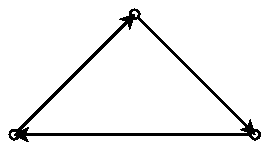
\includegraphics[height=0.3\paperheight]{images/Triangle/Triangle.pdf}
		\end{center}
		A \textit{triangle} is a directed cycle of length three. 
		\uncover<2->{
		\begin{align*}
			\Delta_{G} := \{& (e_1, e_2, e_3) \in E(G)^3 | \\
			 		       & \exists v_1 \neq v_2 \neq v_3 \in V(G): \\
					       & e_1 = (v_1, v_2) \land e_2 = (v_2, v_3) \land e_3 = (v_3, v_1) \} 
		\end{align*} 
		}
	\end{frame}
	
	\begin{frame}[fragile]{Reduction FAST.1}
		If an edge \(e\) is contained in at least \(k+1\) triangles, then reverse \(e\) and reduce \(k\) by \(1\). \newline 
		%TODO: include graphics to explain ?
		\uncover<2->{
		\begin{center}
		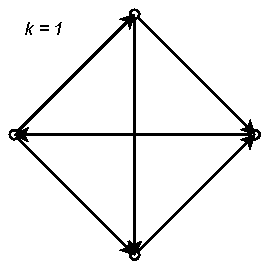
\includegraphics[height=0.5\paperheight]{images/FAST_1/Triangle2.pdf}
		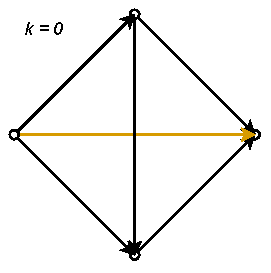
\includegraphics[height=0.5\paperheight]{images/FAST_1/Triangle2Rev.pdf}
		\end{center}
		}
	\end{frame}
	
	\begin{frame}[fragile]{Reduction FAST.1 - Safeness}
		If an edge \(e\) is contained in at least \(k+1\) triangles, then reverse \(e\) and reduce \(k\) by \(1\). \newline 
		\newline
		Let \((G,k)\) be an instance of FAST and
		\[FAS_{(G,k)} := \{ E' \subset E(G) | \text{E' Feedback Arc Set of G} \land \abs{E'} \leq k \} \]
		\only<2>{ 
		\begin{align*}
		& \mathbb{A}: \exists e \in G(E) \text{ contained in at least } k+1 \text{ triangles } \\
		& \Rightarrow \forall F \in FAS_{(G,k)} : e \in F
		\end{align*} 
		}
		\only<3>{
		\begin{align*}
		& \mathbb{A}: (G,k) \in FAST  \\
		& \Rightarrow \exists F \in FAS_{(G,k)} : e \in F \\
		& \Rightarrow F \setminus \{e\} \in FAS_{(G \circledast \{e\},k-1)}  \\
		& \Rightarrow (G',k') = (G \circledast \{e\},k-1) \in FAST
		\end{align*}
		}
	\end{frame}
	
	\begin{frame}[fragile]{Reduction FAST.1 - Safeness}
		Let \((G',k') = (G \circledast \{e\}, k-1) \) be an instance of FAST and
		\[FAS_{(G,k)} := \{ E' \subset E(G) | \text{E' Feedback Arc Set of G} \land \abs{E'} \leq k \} \]
		
		\uncover<2->{
		\begin{align*}
		& \mathbb{A}: \exists F' \in FAS_{(G',k')}: rev(e) \in F' \\
		& \Rightarrow F' \setminus rev\{e\} \in FAS_{(G' \circledast rev\{e\},k')} \\
		& \Rightarrow F' \setminus rev\{e\} \in FAS_{(G, k)} \\
		& \Rightarrow \exists F \in FAS_{(G, k)}: e \neq F \Rightarrow \text{Contradiction!} \\ 
		\end{align*}
		}
	\end{frame}
	
	\begin{frame}[fragile]{Reduction FAST.1 - Safeness}
		Let \((G',k') = (G \circledast \{e\}, k-1) \) be an instance of FAST and
		\[FAS_{(G,k)} := \{ E' \subset E(G) | \text{E' Feedback Arc Set of G} \land \abs{E'} \leq k \} \]
	
		\begin{align*}
		& \Rightarrow \forall F' \in FAS_{(G',k')}: rev(e) \notin F' \\ 
		\\
		\uncover<2->{
		& \mathbb{A}: (G',k') \in FAST \\
		& \Rightarrow \exists F' \in FAS_{(G',k')}: rev(e) \notin F' \\
		& \Rightarrow \exists F' \in FAS_{(G',k')}: F' \cup \{e\} \in FAS_{(G' \circledast rev\{e\},k'+1)} \\
		& \Rightarrow (G,k) = (G' \circledast rev\{e\},k'+1) \in FAST
		}
		\end{align*}
	\end{frame}
	
	\begin{frame}[fragile]{Reduction FAST.1 - Polynomial time}
		\begin{algorithm}[H]
		\only<1-2>{
		\KwData{\( (G, k) \) instance of FAST}
		\KwResult{\( (G', k') \) reduced instance of FAST}
		\BlankLine
		}
		\only<1>{
		$\Delta := \{ \}$\;
		\For{$e_1 = (u_1, v_1) \in E(G)$}{
			\For{$e_2 = (u_2, v_2) \in E(G) \setminus \{e_1\}$}{
				\For{$e_3 = (u_3, v_3) \in E(G) \setminus \{e_1, e_2\}$}{
					\If{$(e_1, e_2, e_3)$ is a triangle, i.e. $v_1 = u_2, v_2 = u_3, v_3 = u_1$}{
						put $(e_1, e_2, e_3)$ in $\Delta$\;
					}
				}
			}
		}
		}
		\only<2->{
		$\Delta = \{(e_1, e_2, e_3) \in E(G)^3 | \exists v_1 \neq v_2 \neq v_3 \in V(G): e_1 = (v_1, v_2) \land e_2 = (v_2, v_3) \land e_3 = (v_3, v_1) \} $\;
		\BlankLine	
		\For{$e \in E(G)$}{
			$k_e \gets 0$\;
			\For{$t \in \Delta$}{
				\If{$e \in t$}{$k_e \gets k_e + 1$\;}
				\If{$k_e \geq k+1$}{\KwRet{$(G \circledast \{e\}, k-1)$}\;}
			}
		}
		\KwRet{$(G,k)$}\;
		}
		\end{algorithm}
		\only<3->{
		\bigskip
		$\Rightarrow$ FAST.1 is computable in polynomial time, e.g. bounded by
		\[ \mathcal{O}(\abs{E(G)}^3) + \mathcal{O}(\abs{E(G)}^4) = \mathcal{O}(\abs{E(G)}^4) \]
		}
	\end{frame}
	
	\begin{frame}[fragile]{Reduction FAST.2}
		If a vertex \(v\) is not contained in any triangle, then delete \(v\) from the tournament.
		\uncover<2->{
		\begin{center}
		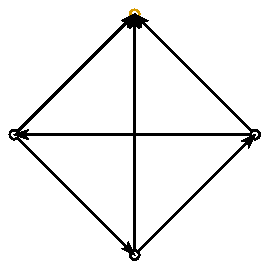
\includegraphics[height=0.5\paperheight]{images/FAST_2/GraphWithVertex.pdf}
		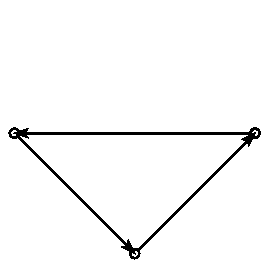
\includegraphics[height=0.5\paperheight]{images/FAST_2/GraphWithoutVertex.pdf}
		\end{center}
		 }
	\end{frame}
	
	\begin{frame}[fragile]{Reduction FAST.2 - Safeness}
		If a vertex \(v\) is not contained in any triangle, then delete \(v\) from the tournament.
		 \begin{align*}
		 & \mathbb{A}: (G,k) \in FAST \\
		 & \Rightarrow \exists F \in FAS_{(G,k)} \\
		 & \Rightarrow F-v \in FAS_{(G,k)} \\
		 & \Rightarrow F-v \in FAS_{(G-v,k)} \\
		 & \Rightarrow (G',k') = (G-v, k) \in FAST
		 \end{align*}
	\end{frame}
	
	\begin{frame}[fragile]{Reduction FAST.2 - Safeness}
		If a vertex \(v\) is not contained in any triangle, then delete \(v\) from the tournament.
   		\begin{align*}
        		& V^{\rightarrow v} := \{u \in V(G) | (u, v) \in E(G) \} \\
        		& V^{\leftarrow v} := \{u \in V(G) | (v, u) \in E(G) \}
        		\end{align*}
		\begin{center}
		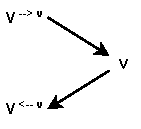
\includegraphics[height=0.3\paperheight]{images/FAST_2/GraphV.pdf}
		\uncover<2->{ 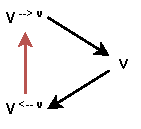
\includegraphics[height=0.3\paperheight]{images/FAST_2/GraphVCircle.pdf} }
		\end{center}
		 \uncover<2->{\[\Rightarrow \nexists (u, w) \in E(G) : u \in V^{\leftarrow v} \land w \in V^{\rightarrow v} \]}
	\end{frame}
	
	\begin{frame}[fragile]{Reduction FAST.2 - Safeness}
		If a vertex \(v\) is not contained in any triangle, then delete \(v\) from the tournament. \\
		\medskip
		\qquad \( \forall V' \subset V(G) : G[ V' ] := (V', \{(u, v) \in E(G) | u, v \in V' \}) \)
		
		\begin{wrapfigure}{R}{0.2\textwidth}
   			\centering
			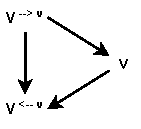
\includegraphics[width = 0.2\textwidth]{images/FAST_2/GraphV2.pdf}
		\end{wrapfigure}
		
		\begin{align*} %TODO: better alignment
		& \mathbb{A}: (G',k') = (G-v, k) \in FAST \\
        		& \Rightarrow \exists F' \in FAS_{(G-v, k)} \\
        		& \Rightarrow F' \cap E(G-v[V^{\rightarrow v}]) \in FAS_{(G-v[V^{\rightarrow v}],n)} \\ 
		& \land F' \cap E(G-v[V^{\leftarrow v}]) \in FAS_{(G-v[V^{\leftarrow v}],m)} \text{ for } n + m = k \\
        		& \Rightarrow F^{\rightarrow v} := F' \cap E(G[V^{\rightarrow v}]) \in FAS_{(G[V^{\rightarrow v}],n)} \\ 
		& \land F^{\leftarrow v} := F' \cap E(G[V^{\leftarrow v}]) \in FAS_{(G[V^{\leftarrow v}],m)} \text{ for } n + m = k \\
        		& \Rightarrow F^{\rightarrow v} \cup F^{\leftarrow v} \in FAS_{(G[V^{\rightarrow v}] \cup G[V^{\leftarrow v}], n + m)} \\
        		& \Rightarrow (G,k) = (G[V^{\rightarrow v}] \cup G[V^{\leftarrow v}], n+m) \in FAST
    		\end{align*}
		
	\end{frame}
	
	\begin{frame}[fragile]{Reduction FAST.2 - Polynomial time}
		\begin{algorithm}[H]
		\only<1-2>{
		\KwData{\( (G, k) \) instance of FAST}
		\KwResult{\( (G', k') \) reduced instance of FAST}
		\BlankLine
		}
		\only<1>{
		$\Delta := \{ \}$\;
		\For{$e_1 = (u_1, v_1) \in E(G)$}{
			\For{$e_2 = (u_2, v_2) \in E(G) \setminus \{e_1\}$}{
				\For{$e_3 = (u_3, v_3) \in E(G) \setminus \{e_1, e_2\}$}{
					\If{$(e_1, e_2, e_3)$ is a triangle, i.e. $v_1 = u_2, v_2 = u_3, v_3 = u_1$}{
						put $(e_1, e_2, e_3)$ in $\Delta$\;
					}
				}
			}
		}
		}
		\only<2->{
		$\Delta = \{(e_1, e_2, e_3) \in E(G)^3 | \exists v_1 \neq v_2 \neq v_3 \in V(G): e_1 = (v_1, v_2) \land e_2 = (v_2, v_3) \land e_3 = (v_3, v_1) \} $\;
		\BlankLine			 
		\For{$v \in V(G)$}{
			\For{$t \in \Delta$}{
				\If{$v \in t$}{\KwCont \;}
			}
			\KwRet{$(G-v,k)$}\;
		}
		\KwRet{$(G,k)$}\;
		}
		\end{algorithm}
		\only<3->{
		\bigskip
		$\Rightarrow$ FAST.2 is computable in polynomial time, e.g. bounded by
		\[ \mathcal{O}(\abs{E(G)}^3) + \mathcal{O}(\abs{V(G)} \cdot \abs{E(G)}^3) + \mathcal{O}(\abs{E(G)}) = \mathcal{O}(\abs{V(G)} \cdot \abs{E(G)}^3) \]
		}
		\end{frame}
	
	\begin{frame}[fragile]{Theorem 2.8 - Proof}
		Let \((G,k) \in FAST\) : neither FAST.1 nor FAST.2 are applicable. \newline \newline
		\(\Rightarrow \exists F \in FAS_{(G,k)} : \)
		\begin{multline*}
			\forall v \in V(G) : \exists t \in \Delta_G, u \in V(G): (v, u) \in t \lor (u, v) \in t 
		\end{multline*}
		\uncover<2>{\begin{multline*} 
			\forall e \in F : \abs{ \{ v \in V(G) | \exists t \in \Delta_G, u \in V(G) : \right. \\ \left. e \in t \land ( (u, v) \in t \lor (v, u) \in t ) \} } \leq k+2
		\end{multline*}
		\begin{center}
			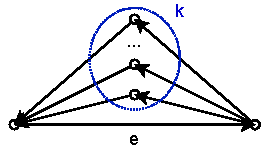
\includegraphics[height = 0.3\pageheight]{images/Theorem28/TrianglesWithE.pdf}
		\end{center}
		}
	\end{frame}
	
	\begin{frame}[fragile]{Theorem 2.8 - Proof}
		Let \((G,k) \in FAST\) : neither FAST.1 nor FAST.2 are applicable. \newline
		\newline
		\(\Rightarrow \exists F \in FAS_{(G,k)} : \) 
		\[\forall v \in V(G) : \exists t \in \Delta_G: e_v \in t \]
		\[ \forall e \in F : \abs{ \{ v \in V(G) | \exists t \in \Delta_G: e \in t \land e_v \in t \} } \leq k+2  \]
		where \( e_v \in t \Leftrightarrow \exists u \in V(G): (v, u) \in t \lor (u, v) \in t \)
		
		\uncover<2->{ 
		\begin{align*}
		\Rightarrow V(G) &= \{v \in V(G) | \exists t \in \Delta_G: e_v \in t \} \\
		&= \{v \in V(G) | \exists e \in F, t \in \Delta_G: e \in t \land e_v \in t \} \\
		&= \bigcup_{e \in F} \{v \in V(G) | t \in \Delta_G: e \in t \land e_v \in t \}
		\end{align*}
		}
		
	\end{frame}
	
	\begin{frame}[fragile]{Theorem 2.8 - Proof}
		Let \((G,k) \in FAST\) : neither FAST.1 nor FAST.2 are applicable. \newline
		\newline
		\(\Rightarrow \exists F \in FAS_{(G,k)} : \) 
		\[\forall v \in V(G) : \exists t \in \Delta_G: e_v \in t \]
		\[ \forall e \in F : \abs{ \{ v \in V(G) | \exists t \in \Delta_G: e \in t \land e_v \in t \} } \leq k+2  \]
		where \( e_v \in t \Leftrightarrow \exists u \in V(G): (v, u) \in t \lor (u, v) \in t \)
		
		\begin{align*} 
		\Rightarrow V(G) &=  \bigcup_{e \in F} \{v \in V(G) | t \in \Delta_G: e \in t \land e_v \in t \} \\
		\only<2->{
		\Rightarrow \abs{V(G)} & \leq \sum_{e \in F} \abs{ \{v \in V(G) | t \in \Delta_G: e \in t \land e_v \in t \} } \\
		& \leq \sum_{e \in F} (k+2) \leq k(k+2) 
		}
		\end{align*}
	\end{frame}
	
	% Define recursive Function for pseudocode
	\RestyleAlgo{ruled}
	\begin{frame}[fragile]{Theorem 2.8 - FAST Kernel}
	\begin{function}[H]
		\caption{Kernel(G, k)}
		\KwData{\( (G, k) \) instance of FAST}
		\KwResult{\( (G', k') \) reduced instance of FAST}
		\BlankLine
		\If{$(G',k') =$ FAST.1$(G,k) \neq (G,k)$}{Kernel(G',k')}
		\If{$(G',k') =$ FAST.2$(G,k) \neq (G,k)$}{Kernel(G',k')}
		\If{$\abs{V(G)} > k(k+2)$}{\KwRet{No-Instance of FAST}}
		\KwRet{$(G,k)$}
	\end{function}
	\only<1>{
	where a No-Instance of FAST might be $(G',k' = 0)$ with
	\begin{gather*}
	V(G') = \{v_1 \neq v_2 \neq v_3 \in V(G)\} \\ E(G') = \{(v_1, v_2), (v_2, v_3), (v_3, v_1) | v_1 \neq v_2 \neq v_3 \in V(G')\}) 
	\end{gather*}
		}
	\only<2->{
	\bigskip
	$\Rightarrow$ FAST Kernel computable in polynomial time, e.g. bounded by
	\[ \mathcal{O}(k \cdot \abs{E(G)}^3) + \mathcal{O}(\abs{V(G)}^2 \cdot \abs{E(G)}^3) = \mathcal{O}(k \cdot \abs{V(G)}^2 \cdot \abs{E(G)}^3) \]
	}
	
	\end{frame}
	
	\begin{frame}[fragile]{Theorem 2.8 - Proof}
		\textit{FAST} admits a kernel with at most \(k^{2} + 2k\) vertices. \newline 
		\newline
		\(\exists\) algorithm \(\mathcal {A}\) returning in \textit{polynomial} time \(\mathcal{A}(G,k) = (G',k'): \)
		\begin{itemize}
			\item \((G,k) \in FAST \Leftrightarrow (G', k') \in FAST \)
			\item \(\abs{V(G')} \leq k(k+2) = k^2 + 2k \)
		\end{itemize}
	\end{frame}
	
\end{document}